%-*- coding:UTF-8 -*-
% gougu.tex
% 勾股定理
%导言区
\documentclass[UTF8]{ctexart}
\title{\heiti 杂谈勾股定理}
\author{\kaishu 张三}
\date{\kaishu 2010年11月5日}
%导入宏包
\usepackage{graphicx}
\usepackage{float}
\usepackage{amsmath}
\usepackage[format=hang,font=small,textfont=it]{caption}%改变图表标题的字体
\usepackage[nottoc]{tocbibind}%增加目录包含项
\newtheorem{thm}{定理}
\newenvironment{myquote}{\begin{quote} \kaishu\zihao{-5}}{\end{quote}}
\newcommand{\degree}{^\circ}

%正文区
\begin{document}
%标题
\maketitle
%摘要
\begin{abstract}
这是一篇关于勾股定理的小短文。
\end{abstract}
%目录
\tableofcontents
%正文内容
%第一部分
\section{勾股定理在古代}
\label{sec:first}
西方称勾股定理为毕达哥拉斯定理,将勾股定理的发现归功于
公元前6世纪的毕达哥拉斯学派\cite{Kline} 。
学派得到了一个法则,可以求出可排成直角三角形三边的三元数组。毕达哥拉斯学派没有书面著作,该定理的严格表述和证明则见于欧几里德\footnote{欧几里德,约公元前330--275 年。}《几何原本》的命题47:“直角三角形斜边上的正方形等于两直角边上的两个正方形之和。”证明是用面积做的。

我国《周髀算经》载商高(约公元前12世纪)答周公问:
\begin{myquote}
勾广三,股修四,径隅五。
\end{myquote}
又载陈子(约公元前7--6 世纪)答荣方问:
\begin{myquote}
若求邪至日者,以日下为勾,日高为股,勾股各自乘,并而开方除之,得邪至日。
\end{myquote}
都较古希腊更早。后者已经明确道出勾股定理的一般形式。图\ref{fig:cherry}是我国古代对勾股
定理的一种证明\cite{quanjing}。
\begin{figure}[ht]
\centering
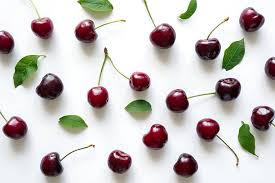
\includegraphics[scale=0.8]{images.jpg}
\caption{樱桃图}
\label{fig:cherry}  
\end{figure}
%第二部分
\section{勾股定理的近似形式}
勾股定理可以用现代语言表述如下:
\begin{thm}[勾股定理]
直角三角形斜边的平方等于两腰的平方和。

可以用符号语言表述为:设直角三角形$ABC$,其中$\angle C=90\degree$,则有
\begin{equation}
\label{eq:gougu}
AB^2 = BC^2 + AC^2
\end{equation}
\end{thm}

满足式\eqref{eq:gougu}的整数成为\emph{勾股数}。第\ref{sec:first}节所说毕达哥拉斯学派得到的三元数组就是勾股数。下表列出一些较小的勾股数:
\begin{table}[h]
\centering
\begin{tabular}{|lll|}
\hline
直角边$a$ & 直角边$b$ & 斜边$c$ \\
\hline
3 & 4 & 5 \\
5 & 12 & 13 \\
\hline
\end{tabular}
\caption{勾股定理}
\end{table}

\bibliographystyle{unsrt}
\nocite{Shiye}
\bibliography{reference}

\end{document}